% Simple plot in TikZ
% Latexdraw.com
% 26/04/2021, 01:25

\documentclass[tikz,border=0.2cm]{standalone}

\begin{document}
	
	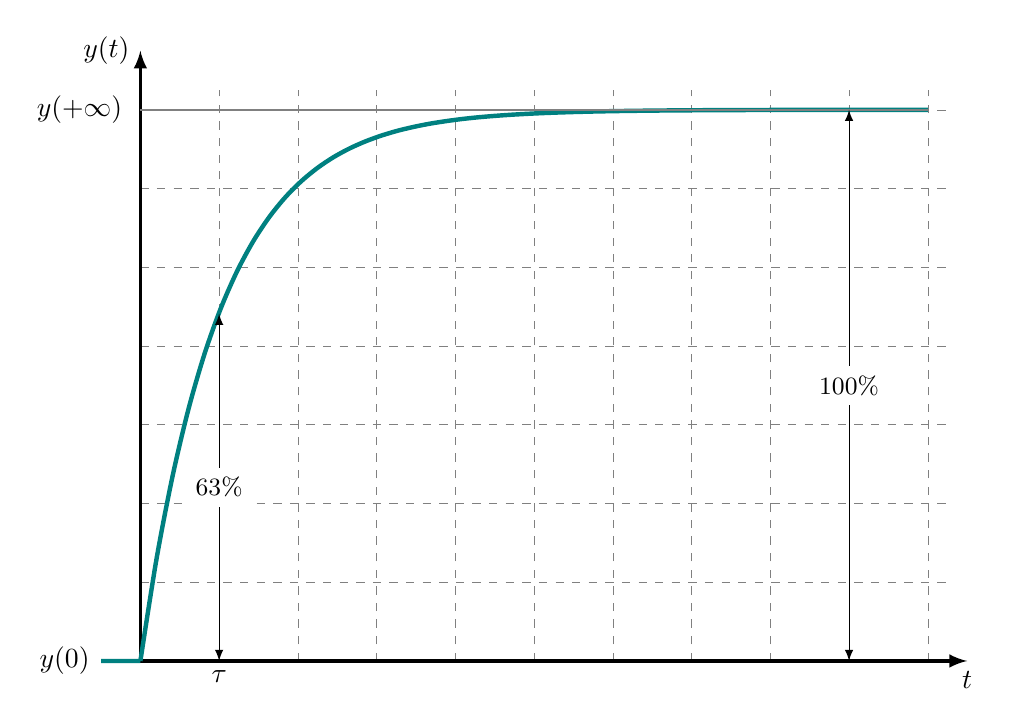
\begin{tikzpicture}
		
		% Grid
		\draw[help lines,dashed] (0,0) grid (10.25,7.25);
		
		% Axes
		\draw[very thick,latex-latex] (0,7.75) node[left]{$y(t)$}
		|- (10.5,0) node[below]{$t$};
		
		% Plot function
		\draw[ultra thick,teal] (-0.5,0) node[left,black](s0){$y(0)$}
		-- ++(0.5,0) 
		plot[domain=0:10,
		samples = 50,
		smooth]({\x}, {7*(1-exp(-\x))});
		
		% y(infty) line 
		\draw[thick,gray] (0,7) node[left=0.1cm,black]{$y(+\infty)$} -- (10,7);
		
		% Line with label 63%
		\draw[latex-latex] (1,0.63*7) -- (1,0) 
		node[below]{$\tau$}
		node[midway,fill=white]{\small $63\%$};
		
		% Lines with label 100%
		\draw[latex-latex] (9,7) -- (9,0)
		node[midway,fill=white]{\small $100\%$};
		
	\end{tikzpicture}
	
\end{document}
